%==============================================================================
%  Multilevel Models for Airbnb Ratings
%  An implementation and extension of Chapter 13, Statistical Rethinking (2nd)
%
%  Compile from this directory with:  pdflatex report.tex   (twice)
%==============================================================================
\documentclass[11pt,a4paper]{article}

\usepackage[T1]{fontenc}
\usepackage[utf8]{inputenc}
\usepackage[margin=1in]{geometry}
\usepackage{amsmath,amssymb}
\usepackage{graphicx}
\usepackage{booktabs}
\usepackage{listings}
\usepackage{xcolor}
\usepackage{caption}
\usepackage{subcaption}
\usepackage[hidelinks]{hyperref}

% figures live one level up, in figures/
\graphicspath{{../figures/}}

%---------------------------- R code formatting ------------------------------
\definecolor{codegray}{gray}{0.95}
\definecolor{codegreen}{rgb}{0.0,0.45,0.15}
\definecolor{codeblue}{rgb}{0.10,0.20,0.65}

\lstdefinestyle{Rstyle}{
  language        = R,
  backgroundcolor = \color{codegray},
  basicstyle      = \ttfamily\footnotesize,
  keywordstyle    = \color{codeblue}\bfseries,
  commentstyle    = \color{codegreen}\itshape,
  stringstyle     = \color{purple},
  breaklines      = true,
  frame           = single,
  framesep        = 4pt,
  rulecolor       = \color{gray},
  showstringspaces= false,
  columns         = flexible,
}
\lstset{style=Rstyle}

%------------------------------ explanation box -------------------------------
\newenvironment{infobox}[1]{%
  \par\vspace{6pt}\begin{center}\begin{minipage}{0.96\textwidth}%
  \rule{\linewidth}{0.8pt}\vspace{3pt}\par
  \textbf{#1}\par\vspace{4pt}\small
}{%
  \par\vspace{3pt}\rule{\linewidth}{0.8pt}%
  \end{minipage}\end{center}\vspace{6pt}\par
}

\title{\textbf{Multilevel Models for Airbnb Ratings}\\[2pt]
       \large An implementation and extension of Chapter 13 of
       \emph{Statistical Rethinking}}
\author{By Tal Ramot, implemented with Claude AI \textcopyright}

\date{}

\begin{document}
\maketitle
\vspace{-2.5em}

%==============================================================================
\section{The problem: a rating is not a measurement}
%==============================================================================

A listing with one review rated $5.0$ is not better than a listing with four
hundred reviews averaging $4.83$. The raw average treats them as equals, and
that is wrong, because the two numbers are not measured with the same
precision.

The data show this before any model is fitted. Across the $70{,}708$ usable
London listings, the \emph{mean} rating barely moves with the number of
reviews, while the \emph{spread} collapses:

\begin{center}
\begin{tabular}{lrrr}
\toprule
reviews & listings & mean rating & SD of rating \\
\midrule
1--2   & 13{,}995 & 4.57 & \textbf{0.865} \\
3--5   & 10{,}615 & 4.66 & 0.496 \\
6--10  &  9{,}959 & 4.70 & 0.341 \\
11--50 & 24{,}332 & 4.74 & 0.239 \\
50+    & 11{,}807 & 4.77 & \textbf{0.179} \\
\bottomrule
\end{tabular}
\end{center}

The spread shrinks by a factor of almost five while the mean moves by two
tenths of a point. If low-review listings were genuinely more variable in
quality, we would expect their mean to move too. It does not. What we are
looking at is sampling noise: an average over two reviews scatters because it
is an average over two reviews.

This is exactly the situation Chapter 13 is about. The chapter's answer is that
each listing should be estimated using \emph{all} the data, not only its own,
and that the amount of information a listing borrows from the others should
depend on how little evidence it has of its own.

%==============================================================================
\section{A generative story, and why it is the Reed frog model}
%==============================================================================

Suppose each review comes from a customer who either had a positive experience
or did not. Let $p_i$ be the probability that an arbitrary customer has a
positive experience at listing $i$, and let the overall rating be the fraction
of positive experiences, rescaled from $[0,1]$ to the star range $[1,5]$. Then
from the observed rating $y_i$ and the review count $N_i$ we can recover a
count of positive reviews:
\[
  p^{\text{obs}}_i = \frac{y_i - 1}{4},
  \qquad
  P_i = \text{round}\!\left(p^{\text{obs}}_i \, N_i\right).
\]
$P_i$ is a count of successes out of $N_i$ trials. That is the tadpole data of
Chapter 13, with \textbf{listings in place of tanks} and \textbf{reviews in
place of tadpoles}. Every listing contributes exactly one row, exactly as every
tank does.

Two assumptions are being made here and it is worth stating them plainly rather
than letting them pass. First, \texttt{review\_scores\_rating} is an average of
one-to-five star ratings, not a proportion of positives; treating it as one is
a modelling choice. Second, \texttt{number\_of\_reviews} counts all reviews,
while the rating is computed only from reviews that carried a score, so $N_i$
slightly overstates the number of trials. Neither changes the structure of the
problem, but both would change the third decimal place.

A note on vocabulary, since it is easy to get backwards: $P_i$ is the
\emph{outcome}, and $\text{Binomial}(N_i, p_i)$ is the \emph{likelihood}. The
prior lives on the intercepts $\alpha_i$, not on $P_i$.

The analysis below uses $200$ listings, $40$ drawn from each of the five review
count bands above, carrying $5{,}563$ reviews between them with a median of $8$
per listing. Stratifying rather than sampling at random is deliberate: a random
sample would be dominated by the middle of the distribution and would contain
too few one-review listings, which are precisely the ones the model is supposed
to do something about.

%==============================================================================
\section{Two models}
%==============================================================================

\paragraph{No pooling.} Every listing gets its own intercept, and the intercepts
know nothing about each other:
\[
  P_i \sim \text{Binomial}(N_i, p_i), \qquad
  \text{logit}(p_i) = \alpha_{\text{listing}[i]}, \qquad
  \alpha_j \sim \text{Normal}(0, 1.5).
\]

\paragraph{Partial pooling.} The prior over the intercepts is itself estimated
from the data:
\[
  P_i \sim \text{Binomial}(N_i, p_i), \qquad
  \text{logit}(p_i) = \alpha_{\text{listing}[i]},
\]
\[
  \alpha_j \sim \text{Normal}(\bar\alpha, \sigma), \qquad
  \bar\alpha \sim \text{Normal}(0, 1.5), \qquad
  \sigma \sim \text{Exponential}(1).
\]

The second model has two more parameters than the first. It will turn out to be
the less flexible of the two, and that apparent contradiction is the whole
lesson.

Model names below follow the book. In the code they are spelled out:
\texttt{m13.1} is \texttt{no\_pooling}, \texttt{m13.1b} is
\texttt{no\_pooling\_flat}, and \texttt{m13.2} is \texttt{partial}, all defined
in \texttt{src/03-models.R}.

\begin{lstlisting}
m13.1 <- ulam(
  alist(
    P ~ dbinom( N , p ),
    logit(p) <- a[listing],
    a[listing] ~ dnorm( 0 , 1.5 )
  ), data=dat , chains=4 , log_lik=TRUE )

m13.2 <- ulam(
  alist(
    P ~ dbinom( N , p ),
    logit(p) <- a[listing],
    a[listing] ~ dnorm( a_bar , sigma ),
    a_bar ~ dnorm( 0 , 1.5 ),
    sigma ~ dexp( 1 )
  ), data=dat , chains=4 , log_lik=TRUE )
\end{lstlisting}

One warning about the fixed prior. Ratings here sit near $4.79$, which means
$p \approx 0.947$ and $\text{logit}(p) \approx 2.9$. A $\text{Normal}(0,1.5)$
prior places the typical listing almost two standard deviations from its own
mean, so it is not a weak prior on this scale; it pulls every listing toward
$p = 0.5$. To check that the comparison below is not an artifact of that, a
third model \texttt{m13.1b} was fitted, identical to \texttt{m13.1} but with
$\alpha_j \sim \text{Normal}(0,5)$, which really is flat.

%==============================================================================
\section{Fitting the model: geometry, not arithmetic}
%==============================================================================

The multilevel model is harder to sample than it looks. The difficulty is that
$\sigma$ and the intercepts are entangled: when $\sigma$ is small, the
$\alpha_j$ must be packed tightly around $\bar\alpha$, and when $\sigma$ is
large they may spread out. The posterior therefore has the shape of a funnel,
narrow at one end and wide at the other, and a step size that suits one end of
the funnel is wrong for the other.

The standard remedy, and the one the chapter gives, is to \emph{reparameterize}.
Instead of sampling the intercepts directly, sample standardized offsets
$z_j \sim \text{Normal}(0,1)$ and rebuild the intercepts from them:
\[
  \alpha_j = \bar\alpha + z_j\,\sigma .
\]
This is the same model. It has the same posterior over $\alpha_j$. But the
parameters the sampler actually moves through, $z_j$, no longer change shape
when $\sigma$ changes, and the funnel goes away.

\begin{lstlisting}
m13.2nc <- ulam(
  alist(
    P ~ dbinom( N , p ),
    logit(p) <- a_bar + z[listing]*sigma,
    z[listing] ~ dnorm( 0 , 1 ),
    a_bar ~ dnorm( 0 , 1.5 ),
    sigma ~ dexp( 1 ),
    gq> vector[listing]:a <<- a_bar + z*sigma
  ), data=dat , chains=4 , log_lik=TRUE )
\end{lstlisting}

Both versions were fitted. The results:

\begin{center}
\begin{tabular}{lrrrr}
\toprule
 & divergent & min E-BFMI & max $\hat{R}$ & min $n_{\text{eff}}$ \\
\midrule
centered      & 0 & \textbf{0.216} & 1.023 & \textbf{150} \\
non-centered  & 0 & \textbf{0.736} & 1.001 & \textbf{714} \\
\bottomrule
\end{tabular}
\end{center}

Neither version produced a single divergent transition, so the warning most
often associated with the funnel never fired. This is worth being honest about:
the textbook symptom did not appear on this data set. The funnel showed up
anyway, in two quieter places. Stan warned that the energy diagnostic E-BFMI
was below $0.3$ on all four chains of the centered model --- it came in at
$0.216$, against $0.736$ after reparameterizing --- and the centered model
extracted only $150$ effectively independent draws of $\sigma$ from the same
$2{,}000$ samples that gave the non-centered model $714$. Reparameterizing
bought nearly a fivefold improvement in the precision of $\sigma$ for no extra
computation, and since everything in Section 9 depends on the $\sigma$
posterior, that matters.

\begin{infobox}{What the diagnostics mean}
\textbf{Divergent transitions.} Stan simulates a physical trajectory across the
posterior. When the surface curves more sharply than the step size can follow,
the simulated trajectory diverges from the true one, and Stan records it. A
divergence means the sampler could not go where it was trying to go, so that
region of the posterior is under-explored. Even a handful is a reason to
distrust the result.

\smallskip
\textbf{E-BFMI} looks at the same problem from the direction of energy. If the
sampler cannot change energy efficiently between iterations, it cannot move
between the narrow and wide parts of a funnel. Values below $0.3$ are a
warning. It catches funnels that produce no divergences at all, which is what
happened here.

\smallskip
\textbf{$\hat{R}$} compares the variance within each chain to the variance
across chains. If the chains have converged to the same distribution, the two
agree and $\hat{R}$ approaches $1$. Values above about $1.01$ mean the chains
have not agreed yet.

\smallskip
\textbf{$n_{\text{eff}}$ (\texttt{ess\_bulk})} is the number of
\emph{effectively independent} samples. Markov chain draws are correlated, so
$2{,}000$ samples are worth fewer than $2{,}000$ independent ones. It is a
measure of how much information the chains actually delivered, not how long
they ran.
\end{infobox}

\subsection{Trace plots}

A trace plot draws each chain's path over the iterations. What we want is what
McElreath calls a fuzzy caterpillar: the chains should sit in the same
horizontal band, wiggle rapidly, and none of them should wander off or stick in
one place for a stretch.

\begin{figure}[h!]
\centering
\textbf{\small (a) centered}\\[2pt]
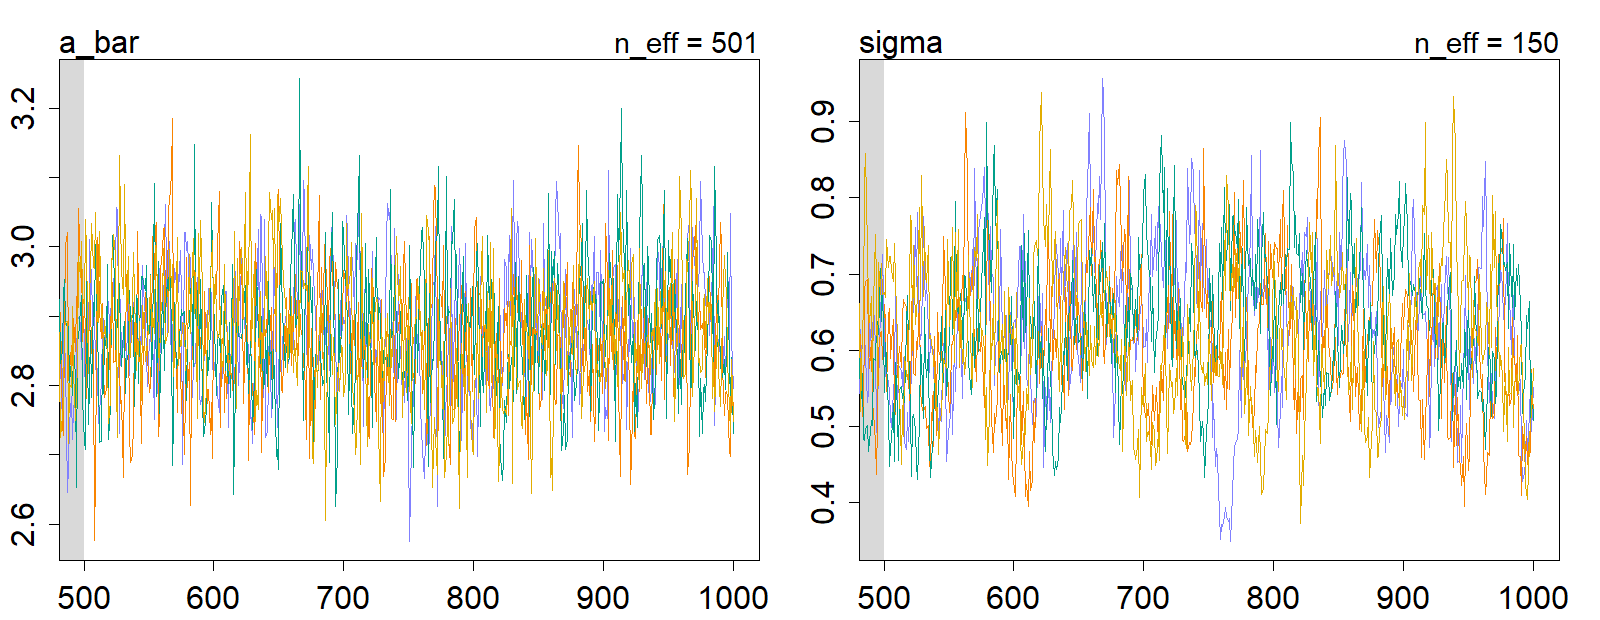
\includegraphics[width=0.92\textwidth]{01-trace-centered.png}\\[6pt]
\textbf{\small (b) non-centered}\\[2pt]
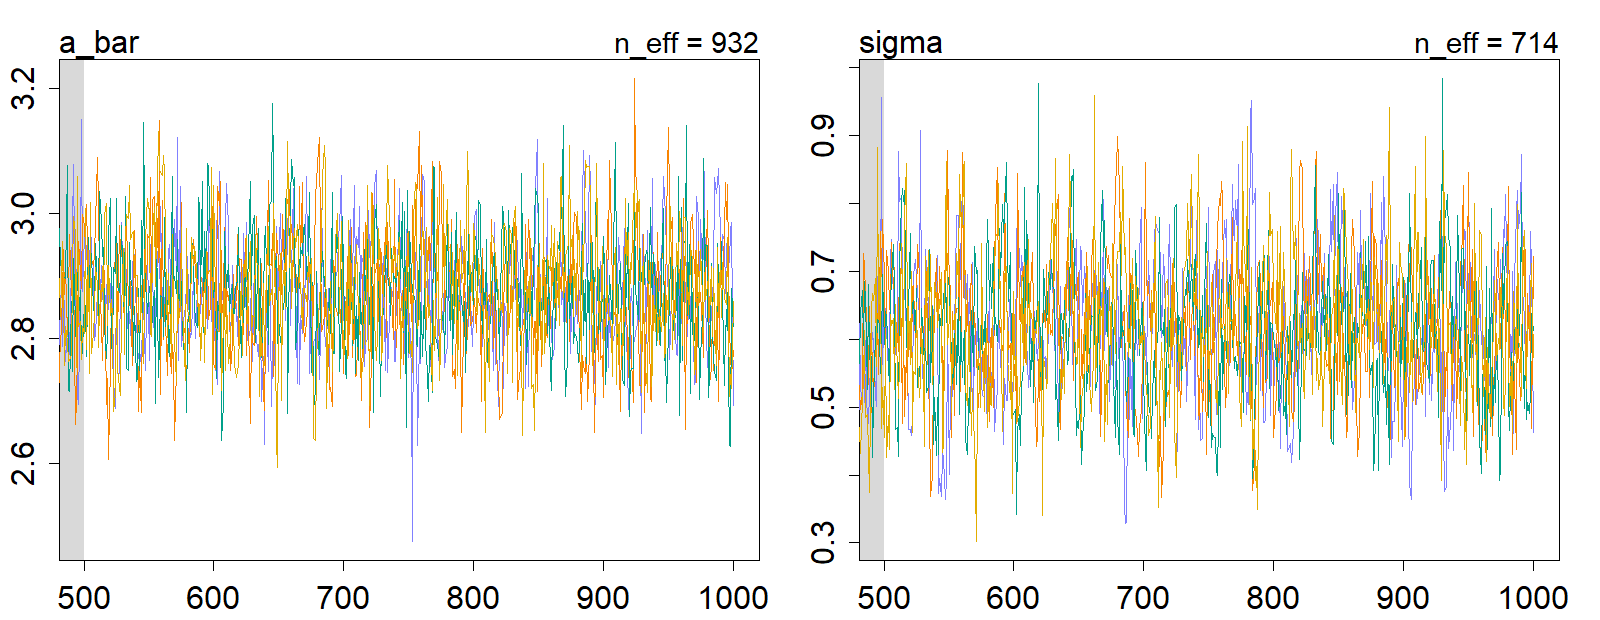
\includegraphics[width=0.92\textwidth]{02-trace-noncentered.png}
\caption{Trace plots for $\bar\alpha$ and $\sigma$, warmup excluded. Both are
stationary --- neither is broken --- but they are not equally good. The
centered $\sigma$ trace makes slow excursions that last tens of iterations,
wandering low for a stretch and then high. The non-centered trace oscillates
rapidly with no such drift. Slow excursions mean successive draws carry nearly
the same information, which is exactly what a low effective sample size
reports.}
\end{figure}

\subsection{Trace rank plots}

Trace plots become hard to read once four chains overlap, because the ink piles
up and a chain that is slightly wrong is hidden behind three that are right. A
trace rank plot fixes this. All the samples from all the chains are ranked
together, from lowest to highest, and then each chain's ranks are histogrammed
separately.

The logic is simple. If every chain is exploring the same distribution, then
each chain should own roughly its fair share of the low ranks, the middle
ranks, and the high ranks. So the histograms should be flat and should overlap.
A chain that is stuck somewhere too long will own too many ranks in one region
and show up as a histogram that rises above the others.

\begin{figure}[h!]
\centering
\textbf{\small (a) centered}\\[2pt]
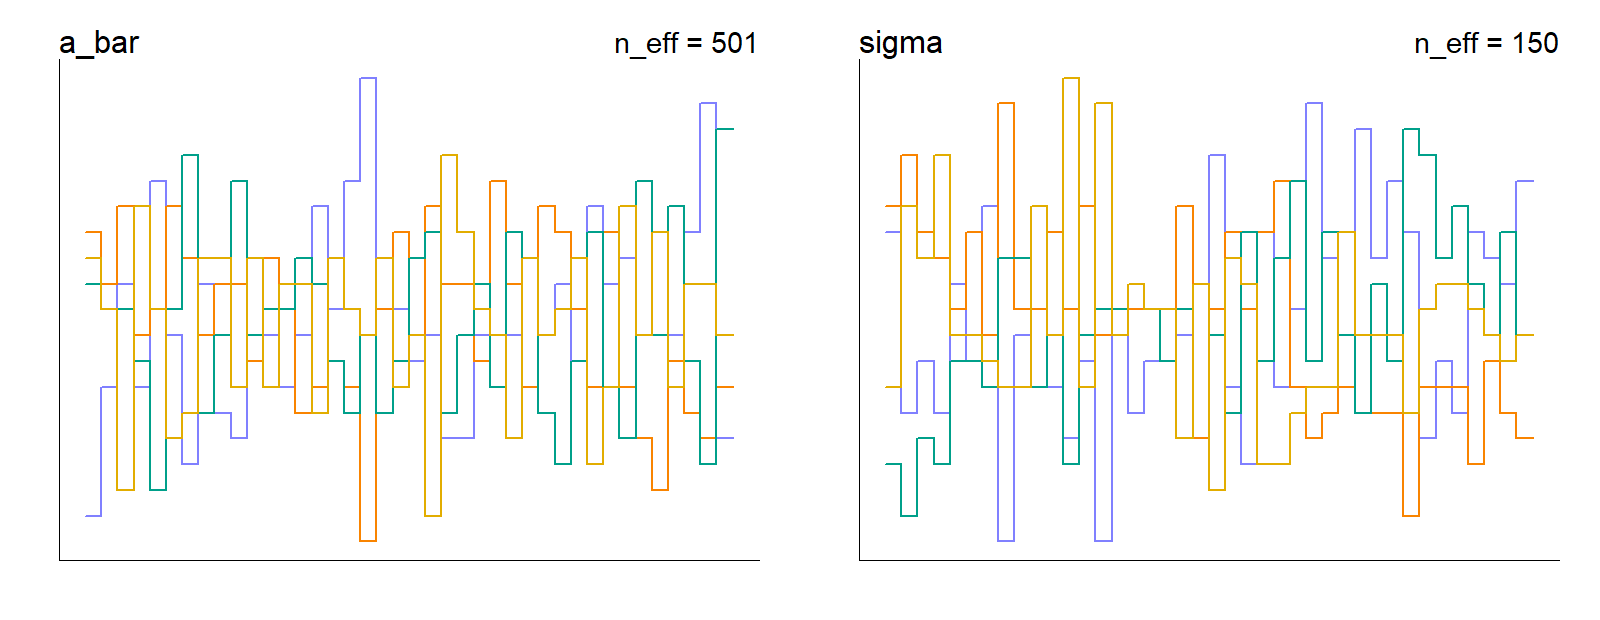
\includegraphics[width=0.92\textwidth]{03-trank-centered.png}\\[6pt]
\textbf{\small (b) non-centered}\\[2pt]
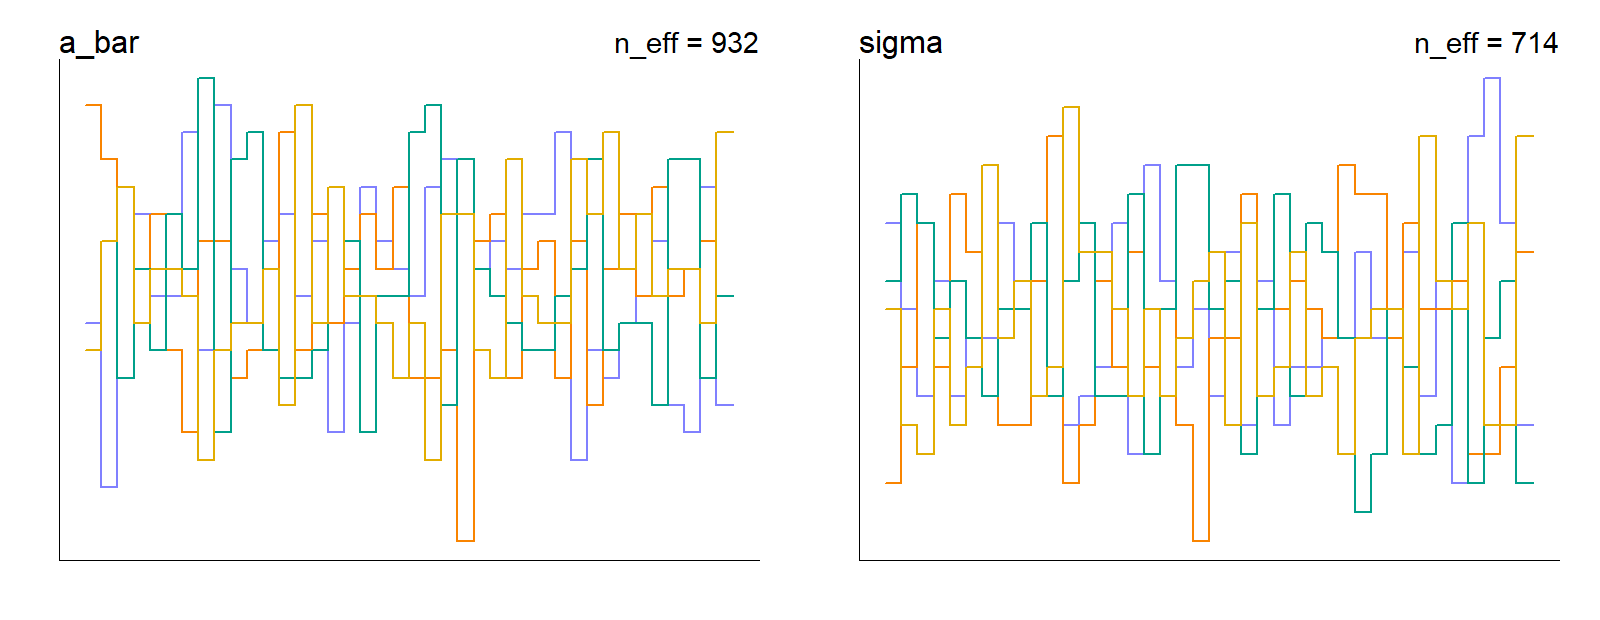
\includegraphics[width=0.92\textwidth]{04-trank-noncentered.png}
\caption{Trace rank plots. Look at the $\sigma$ panel of (a): one chain holds
far more than its share of the lowest ranks at the left edge, and another
spikes at the highest ranks on the right. Those are chains that spent too long
in one region --- the same slow excursions the trace plot showed, now visible
as an imbalance rather than as a wiggle. In (b) the four histograms interleave
much more evenly.}
\end{figure}

%==============================================================================
\section{What the model estimates}
%==============================================================================

\begin{table}[h!]
\centering
\begin{tabular}{lrrrrrr}
\toprule
 & mean & sd & 5.5\% & 94.5\% & $\hat{R}$ & $n_{\text{eff}}$ \\
\midrule
\texttt{a\_bar} & 2.876 & 0.094 & 2.730 & 3.031 & 1.001 & 932 \\
\texttt{sigma}  & 0.617 & 0.103 & 0.456 & 0.786 & 1.001 & 714 \\
\bottomrule
\end{tabular}
\caption{\texttt{precis(m13.2, depth=1)}. The 200 listing intercepts are
hidden; \texttt{depth=2} would show them all.}
\end{table}

Reading this table: \texttt{mean} and \texttt{sd} describe the marginal
posterior of each parameter, and the two percentage columns give the $89\%$
compatibility interval. The last two columns are the diagnostics from the box
above, and both are healthy here.

The numbers themselves say two things. $\bar\alpha = 2.88$ on the log-odds
scale is $\text{logit}^{-1}(2.88) = 0.947$ as a probability, or $1 + 4(0.947) =
4.79$ on the star scale. That is the average listing, and it matches the
population mean of the full data set. And $\sigma = 0.62$ says how far listings
genuinely differ from one another once sampling noise has been accounted for.
It is not zero, so listings really do vary; it is also well below $1.5$, which
is the fixed prior the no-pooling model was using, and that comparison is what
decides the next section.

%==============================================================================
\section{Comparing the models}
%==============================================================================

\begin{table}[h!]
\centering
\begin{tabular}{lrrrrr}
\toprule
 & WAIC & SE & dWAIC & dSE & \textbf{pWAIC} \\
\midrule
\texttt{m13.2}  multilevel        & 485.1 & 28.4 &   0.0 & --   & \textbf{37.5} \\
\texttt{m13.1b} no pooling, flat  & 508.3 & 25.7 &  23.2 & 14.7 & 73.3 \\
\texttt{m13.1}  no pooling, book  & 690.2 & 18.3 & 205.1 & 18.7 & 112.1 \\
\bottomrule
\end{tabular}
\caption{\texttt{compare(m13.1, m13.1b, m13.2)}.}
\end{table}

\begin{infobox}{WAIC and pWAIC}
\textbf{WAIC} estimates how well a model will predict data it has not seen. It
takes the fit to the data it \emph{has} seen and subtracts a penalty for
flexibility. Lower is better, and only differences between models on the same
outcome mean anything --- the absolute value does not.

\smallskip
\textbf{pWAIC} is that penalty: the \emph{effective number of parameters}. It is
computed from how much the log-likelihood of each observation varies across the
posterior. A parameter that is pinned down by the data, or held in place by a
tight prior, contributes little. A parameter free to chase its own data point
contributes about one. So pWAIC counts not how many parameters a model has, but
how many it is really \emph{using}.

\smallskip
\textbf{dWAIC} is the difference from the best model and \textbf{dSE} is the
standard error of that difference --- the number to compare it against.
\end{infobox}

The pWAIC column is the point of the whole exercise. The multilevel model has
$202$ parameters. The no-pooling models have $200$. Yet the multilevel model
uses the equivalent of $37.5$ of them, against $73.3$ and $112.1$. It is the
model with the most parameters and the least overfitting.

The reason is the adaptive prior. In \texttt{m13.1} each intercept is regularized
by a fixed $\text{Normal}(0,1.5)$ that was chosen before seeing any data. In
\texttt{m13.2} the model learns from the data that the true spread is
$\sigma = 0.62$, which is far tighter, and applies that. Regularization the
model works out for itself beats regularization we guessed in advance.

The sensitivity fit is worth a sentence, because it comes out backwards from
what one might expect. \texttt{m13.1b}, with the \emph{wider} prior, has the
\emph{lower} pWAIC of the two no-pooling models. The reason is that
$\text{Normal}(0,1.5)$ is not merely tight, it is tight \emph{in the wrong
place}: it is centered on $p = 0.5$ while the data sit at $p = 0.947$. Prior
and likelihood pull against each other for every listing, and that conflict
inflates the variance of the log-likelihood, which is what pWAIC measures. The
comparison survives either way --- $37.5$ beats both --- so the multilevel
model's advantage is not an artifact of the prior we happened to choose.

%==============================================================================
\section{The population of listings}
%==============================================================================

A multilevel model does not only estimate $200$ intercepts. It estimates the
\emph{distribution} those intercepts were drawn from, and that is what allows it
to say anything at all about a listing it has never seen.

\begin{figure}[h!]
\centering
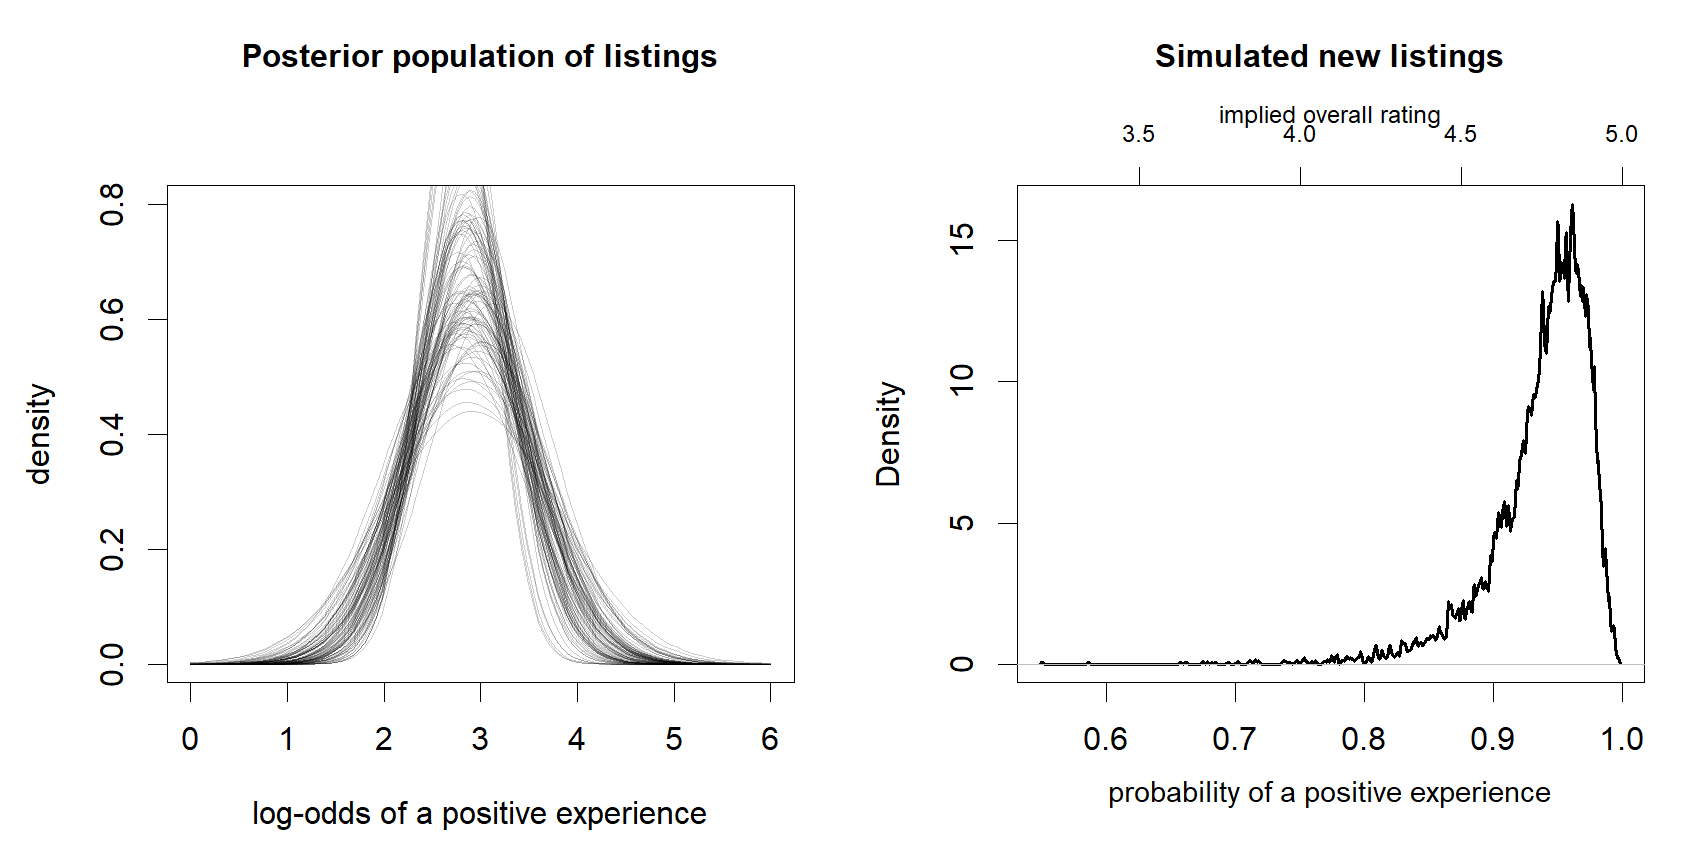
\includegraphics[width=0.95\textwidth]{05-population.png}
\caption{Left: one hundred draws of the population distribution of listings on
the log-odds scale, each curve a $\text{Normal}(\bar\alpha, \sigma)$ using one
posterior sample. The spread of the curves is uncertainty about the population;
the width of each curve is the variation among listings. Right: $8{,}000$
simulated listings pushed through the inverse logit, so the horizontal axis is
the probability of a positive experience, with the implied star rating marked
on top.}
\end{figure}

\begin{lstlisting}
post <- extract.samples( m13.2 )
plot( NULL , xlim=c(0,6) , ylim=c(0,0.8) ,
      xlab="log-odds of a positive experience" , ylab="density" )
for ( i in 1:100 )
    curve( dnorm(x,post$a_bar[i],post$sigma[i]) , add=TRUE ,
           col=col.alpha("black",0.2) )

sim_listings <- rnorm( 8000 , post$a_bar , post$sigma )
dens( inv_logit(sim_listings) , lwd=2 , adj=0.1 )
\end{lstlisting}

The transformation matters. On the log-odds scale the population is a symmetric
bell. On the probability scale it is strongly skewed, piled up near $1$ with a
long tail reaching down. That asymmetry is not something we assumed; it is what
a symmetric distribution becomes once it is squeezed through the inverse logit
near the top of its range. It is also a fair description of Airbnb: most
listings are fine, and the interesting variation is all on the downside.

%==============================================================================
\section{Shrinkage}
%==============================================================================

\begin{figure}[h!]
\centering
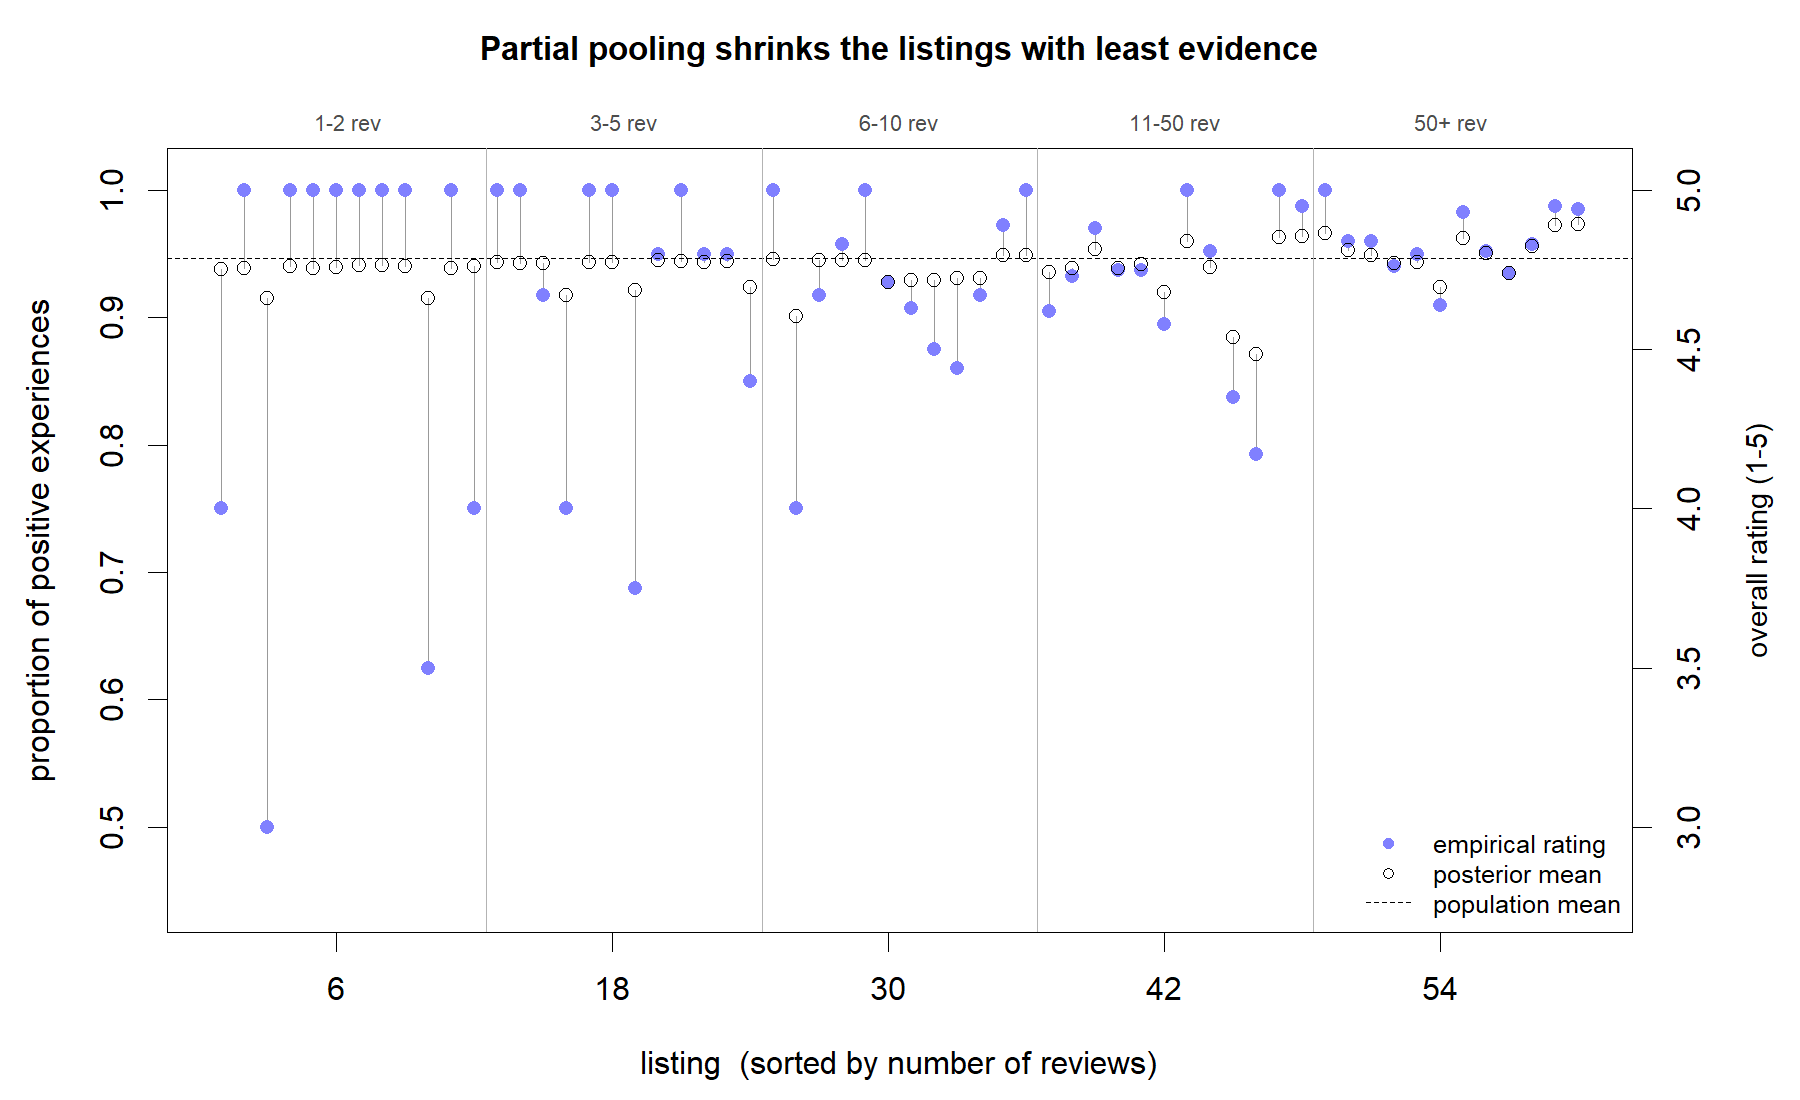
\includegraphics[width=\textwidth]{06-shrinkage.png}
\caption{Filled points are the empirical ratings, open points the posterior
means, and the segment between them is what pooling did. The dashed line is the
population mean $\text{logit}^{-1}(\bar\alpha)$. Listings are sorted by review
count, with the bands marked along the top.}
\end{figure}

The picture is the one Chapter 13 promises. On the left, where listings have one
or two reviews, the segments are long and every one of them points toward the
dashed line. On the right, where listings have fifty reviews or more, the open
and filled points sit on top of each other. Nothing was done to the model to
produce this gradient. It follows from the binomial likelihood: a count out of
$400$ trials is sharp evidence and overwhelms the prior, while a count out of
one trial is almost no evidence and the prior wins.

\begin{table}[h!]
\centering
\begin{tabular}{lrrrr}
\toprule
reviews & mean shift & spread before & spread after & \textbf{shrink factor} \\
\midrule
1--2   & 0.327 & 0.314 & 0.032 & \textbf{0.899} \\
3--5   & 0.396 & 0.445 & 0.059 & 0.869 \\
6--10  & 0.214 & 0.257 & 0.045 & 0.826 \\
11--50 & 0.111 & 0.168 & 0.063 & 0.625 \\
50+    & 0.047 & 0.116 & 0.070 & \textbf{0.395} \\
\bottomrule
\end{tabular}
\caption{All quantities in rating points. ``Spread'' is the mean distance from
the population mean, before and after pooling; the shrink factor is
$1 - \text{after}/\text{before}$.}
\end{table}

One column in that table is not monotone and the reason is instructive. The
mean shift for one-to-two-review listings ($0.327$) is \emph{smaller} than for
three-to-five ($0.396$). This is not an error. A listing with a single review is
almost always rated exactly $5.0$, and $5.0$ is only about $0.2$ rating points
above the population mean of $4.79$, so there is very little distance to travel
even though nearly all of it is taken away. The shrink factor, which measures
the \emph{fraction} of the gap that pooling closes, is the honest summary, and
it falls monotonically from $0.90$ to $0.40$.

%==============================================================================
\section{Extension: what is $\sigma$ actually doing?}
%==============================================================================

Everything above rests on a claim that Chapter 13 makes but does not check: that
$\sigma$ is a regularization strength, and that the model chooses a good one.
That claim is testable.

If $\sigma$ really is a regularizer, then fixing it by hand at the value the
model chose ought to predict new data better than fixing it anywhere else. So:
refit the multilevel model twelve times with $\sigma$ \emph{pinned} at values
from $0.15$ to $2.5$, leaving $\bar\alpha$ free, and score each fit by
cross-validation. If the claim holds, the cross-validation curve should peak
where the posterior of $\sigma$ peaked in the model that estimated it.

\begin{lstlisting}
sigma_grid <- exp( seq( log(0.15) , log(2.5) , length.out=12 ) )

for ( i in seq_along(sigma_grid) ) {
    dat_s <- c( dat , list( sigma_fixed=sigma_grid[i] ) )
    fits[[i]] <- ulam(
      alist(
        P ~ dbinom( N , p ),
        logit(p) <- a[listing],
        a[listing] ~ dnorm( a_bar , sigma_fixed ),
        a_bar ~ dnorm( 0 , 1.5 )
      ), data=dat_s , chains=4 , log_lik=TRUE )
}
\end{lstlisting}

\subsection{Cross-validation needs care here}

The obvious tool is \texttt{PSIS}, and the obvious tool is the wrong one. Every
listing contributes exactly one observation, so dropping listing $i$ removes
\emph{all} the information about $\alpha_i$. PSIS estimates what would happen if
we dropped a point by reweighting a posterior that was fitted \emph{with} that
point, and when the point is the only thing holding a parameter in place, that
reweighting is being asked to do far too much. The Pareto $k$ diagnostic says so
loudly: essentially every point is flagged.

But the same fact that breaks PSIS makes the exact answer easy. With $\alpha_i$
unconstrained by the remaining data, the leave-one-out prediction for listing
$i$ is just the prediction for a brand new listing:
\[
  p(P_i \mid y_{-i}, \sigma)
  = \int \text{Binomial}\big(P_i \mid N_i, \text{logit}^{-1}(a)\big)\,
         \text{Normal}(a \mid \bar\alpha, \sigma)\, da ,
\]
averaged over the posterior of $\bar\alpha$. This needs no importance sampling
at all --- draw $\bar\alpha$ from the posterior, draw $a$ around it, average the
binomial density. It handles $\alpha_i$ exactly. Its only approximation is that
it reuses the full-data posterior of $\bar\alpha$ rather than refitting without
listing $i$, which moves $\bar\alpha$ by a fraction of its own posterior
standard deviation when one listing in two hundred is removed.

\subsection{The result}

\begin{table}[h!]
\centering
\begin{tabular}{rrrrr}
\toprule
$\sigma$ & elpd PSIS & bad $k$ & elpd WAIC & \textbf{elpd direct} \\
\midrule
0.150 & $-268.0$ &  2 & $-267.6$ & $-265.7$ \\
0.194 & $-265.2$ &  4 & $-264.5$ & $-263.1$ \\
0.250 & $-260.6$ &  3 & $-259.3$ & $-260.0$ \\
0.323 & $-257.1$ &  7 & $-254.2$ & $-256.8$ \\
0.417 & $-252.3$ &  6 & $-248.7$ & $-253.9$ \\
\textbf{0.539} & $-249.4$ & 16 & $-244.1$ & $\mathbf{-252.2}$ \\
\textbf{0.696} & $\mathbf{-247.0}$ & 27 & $-240.0$ & $-252.3$ \\
0.899 & $-247.4$ & 36 & $-238.1$ & $-255.3$ \\
\textbf{1.161} & $-248.2$ & 45 & $\mathbf{-237.2}$ & $-261.8$ \\
1.499 & $-252.4$ & 58 & $-237.7$ & $-272.2$ \\
1.936 & $-257.7$ & 72 & $-239.7$ & $-286.6$ \\
2.500 & $-264.4$ & 97 & $-241.9$ & $-304.4$ \\
\bottomrule
\end{tabular}
\caption{Each row is a separate model with $\sigma$ pinned. Higher elpd is
better; the best value in each column is bold. ``bad $k$'' counts the listings,
out of $200$, whose Pareto $k$ exceeds $0.7$ --- the diagnostic that says PSIS
should not be believed.}
\end{table}

\begin{figure}[h!]
\centering
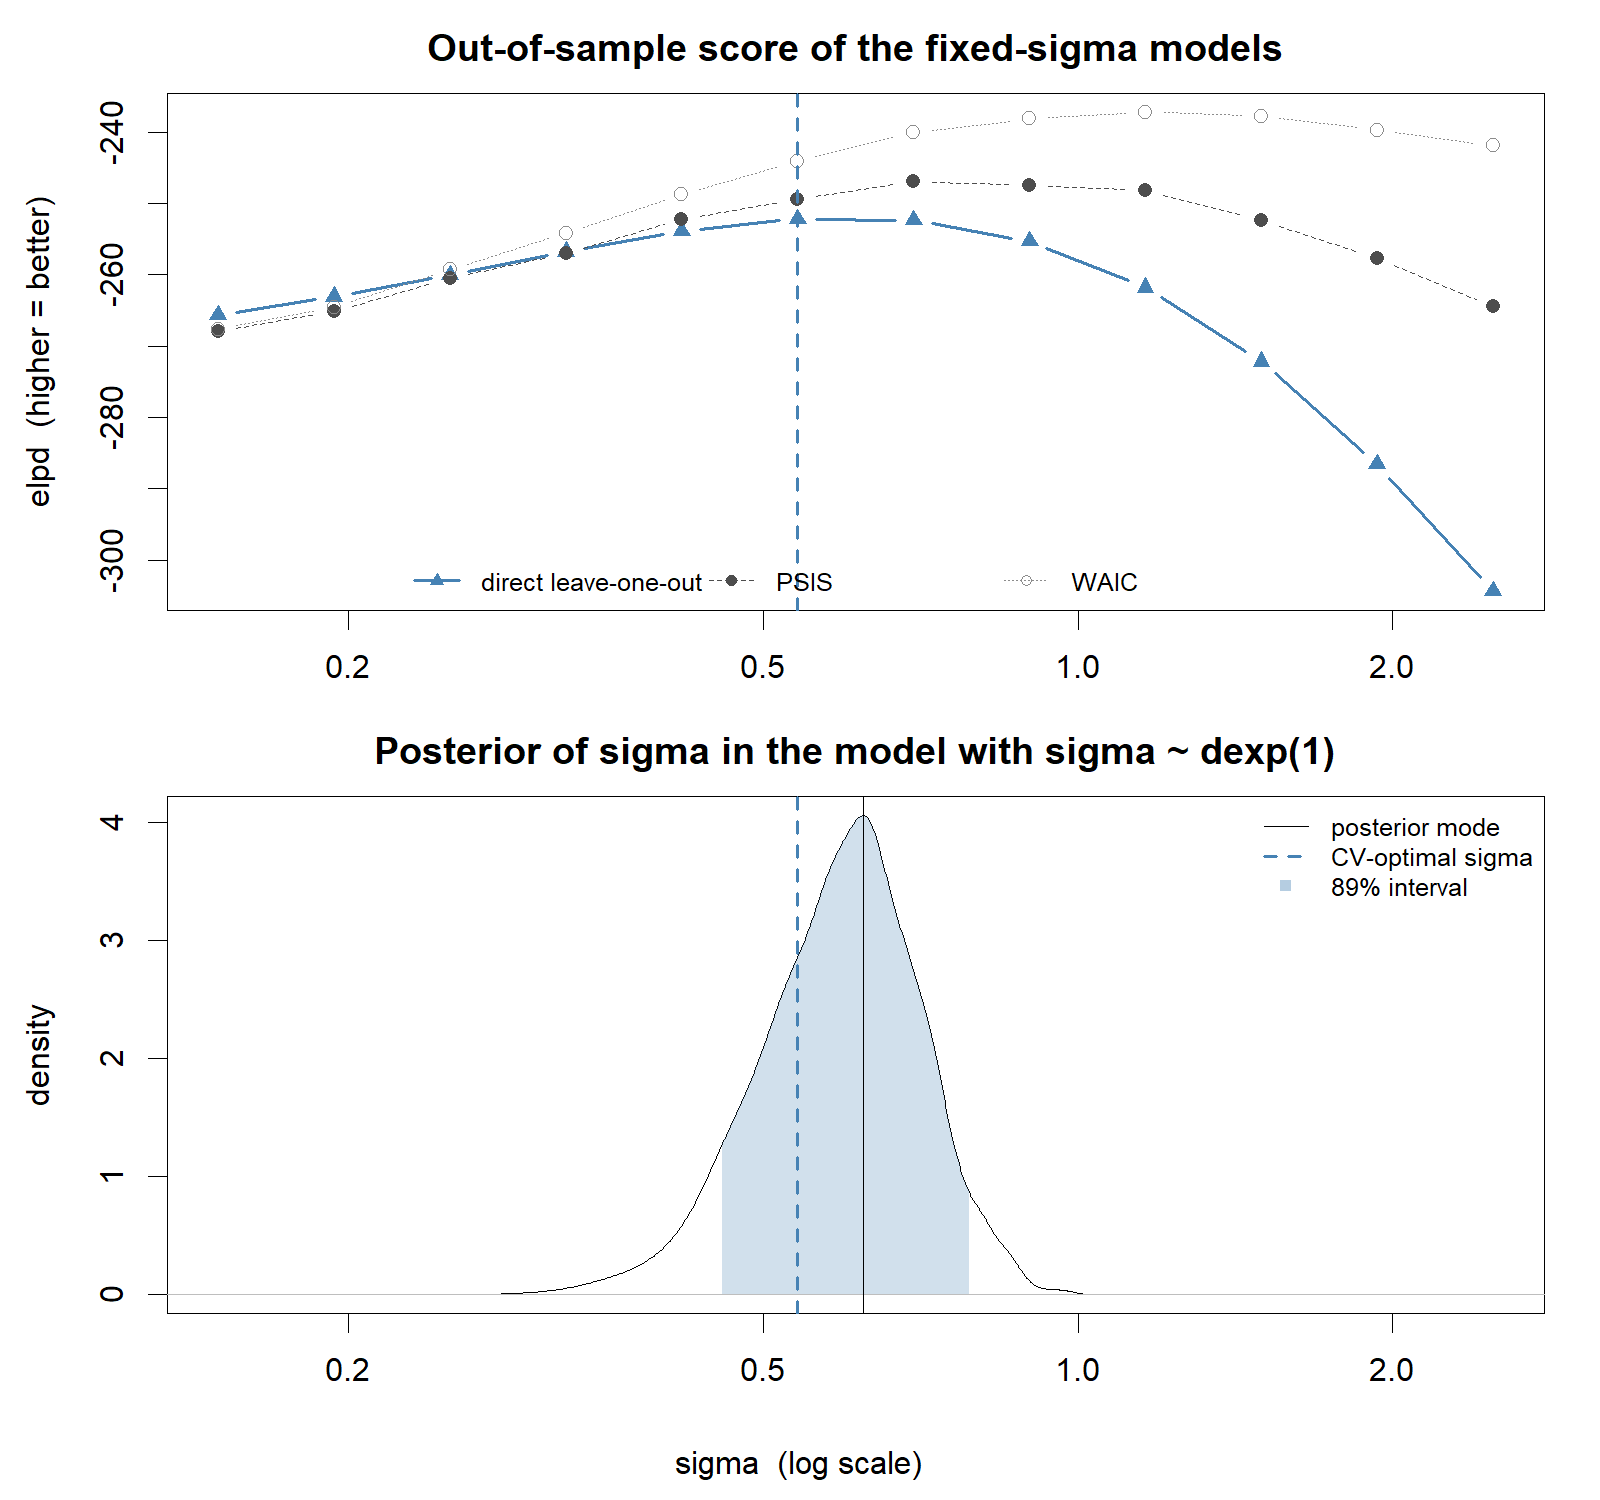
\includegraphics[width=0.9\textwidth]{07-sigma-agreement.png}
\caption{Top: out-of-sample score of each fixed-$\sigma$ model, by three
criteria. Bottom: the posterior of $\sigma$ from the model that estimated it
with a $\text{Exponential}(1)$ prior, with its $89\%$ interval shaded. The
dashed line is the cross-validation optimum, carried down from the top panel.}
\end{figure}

\textbf{The direct cross-validation curve and the posterior land in the same
place.} The curve is highest at $\sigma = 0.539$, with $\sigma = 0.696$ all but
tied ($-252.2$ against $-252.3$), and the posterior mode of $0.623$ falls
between those two adjacent grid points. Both sit comfortably inside the $89\%$
interval $[0.456, 0.786]$.

A purely predictive criterion, which knows nothing about priors, and a purely
Bayesian one, which never simulated a held-out data point, choose the same
amount of pooling. The multilevel model found by regularization what
cross-validation found by brute force.

Three honest caveats. The two quantities are not required to agree
\emph{exactly}: they optimize related but different objectives, and the
$\text{Exponential}(1)$ prior pulls the posterior mode slightly down relative to
the cross-validation optimum. The grid is coarse, so it locates the optimum
only to the nearest grid point. And the peak is \emph{flat}, so the data do not
distinguish sharply between nearby amounts of pooling. What the curve does say
sharply is that both ends are bad: pinning $\sigma$ at $0.15$ costs $13$ elpd
and pinning it at $2.5$ costs $52$. The claim is agreement, not identity.

The disagreement between the criteria is a result in its own right. Both PSIS
and WAIC peak at \emph{larger} $\sigma$ than the direct computation --- one grid
step for PSIS, three for WAIC --- that is, they recommend \emph{less} pooling
than is good for prediction. The reason is the same one that made PSIS
unreliable: both estimate the cost of a held-out point using a posterior in
which that point's own parameter was fitted to it. They therefore undercount how
much flexibility the model is using, and a model whose flexibility is
undercounted looks like it can afford more.

The bad-$k$ column tracks the damage. It climbs from $2$ at $\sigma = 0.15$ to
$97$ at $\sigma = 2.5$, and stands at $27$ at the very $\sigma$ that PSIS
nominates --- the diagnostic is loudest exactly where the answer is being read
off. The direct computation has no such blind spot. It is a useful reminder that
an information criterion is an approximation, and that approximations have
assumptions --- one observation per cluster violates this one.

%==============================================================================
\section{Conclusion}
%==============================================================================

Starting from the observation that a rating computed from two reviews is not the
same kind of number as a rating computed from four hundred, we wrote down a
generative story in which reviews are trials and ratings are proportions, and
that story turned out to be the Reed frog model. Fitting it required attention
to the geometry of the posterior rather than to the model itself: the
reparameterization $\alpha_j = \bar\alpha + z_j \sigma$ changes nothing about
what is being estimated and everything about how well it can be estimated.

The comparison delivered the chapter's central result. The multilevel model has
two more parameters than the no-pooling model and uses a third as many of them,
because it learned its own regularization instead of being handed one. The
shrinkage plot showed where that regularization goes: almost entirely onto the
listings with the least evidence, and almost not at all onto the listings with
the most.

Finally, pinning $\sigma$ by hand and scoring the result by cross-validation
confirmed that the $\sigma$ the model estimates is the $\sigma$ that predicts
best. Along the way it also showed that the standard tools for that scoring,
PSIS and WAIC, cannot be trusted when every cluster holds a single observation
--- which is worth knowing, because it is a common shape for data to have.

\end{document}
